\documentclass{article}
\usepackage{listings}
\usepackage{xcolor}
\usepackage[a4paper, margin=0.55in, top=0.5in]{geometry}
\usepackage{hyperref}
\usepackage{graphicx} % Required for including images and using \centering

\lstset{
    basicstyle=\ttfamily\footnotesize,
    keywordstyle=\color{blue}\bfseries,
    commentstyle=\color{gray},
    stringstyle=\color{red},
    showstringspaces=false,
    breaklines=true,
    frame=single,
    numbers=left,
    numberstyle=\tiny,
    numbersep=5pt,
    tabsize=2
}

\begin{document}

\title{Plotting Histograms Using \texttt{plot\_all.py}}
\author{Ibrahim H.I. Abushawish}
\maketitle
\section*{Plotting Histograms Using \texttt{plot\_all.py}}
The process of plotting histograms over each other using the provided \texttt{plot\_all.py} script involves the following steps:

The files to combine are determined based on the reference tutorial for the analysis, as outlined in the following links:
\begin{itemize}
    \item {\scriptsize \url{https://github.com/atlas-outreach-data-tools/atlas-outreach-cpp-framework-13tev/blob/688d73fb73a742a4e43912189411dcae4dec85e2/Plotting/Plotting.cxx}}
    \item {\scriptsize \url{https://github.com/atlas-outreach-data-tools/atlas-outreach-cpp-framework-13tev/blob/master/Plotting/Plotting.cxx}}
\end{itemize}

These files should be combined with proper naming conventions to match the expected input of the \texttt{plot\_all.py} script. Ensure that the combined files are named appropriately (e.g., \texttt{data.root}, \texttt{V.root}, \texttt{VV.root}, etc.) to align with the script's requirements.


\begin{figure}[h]
    \centering
    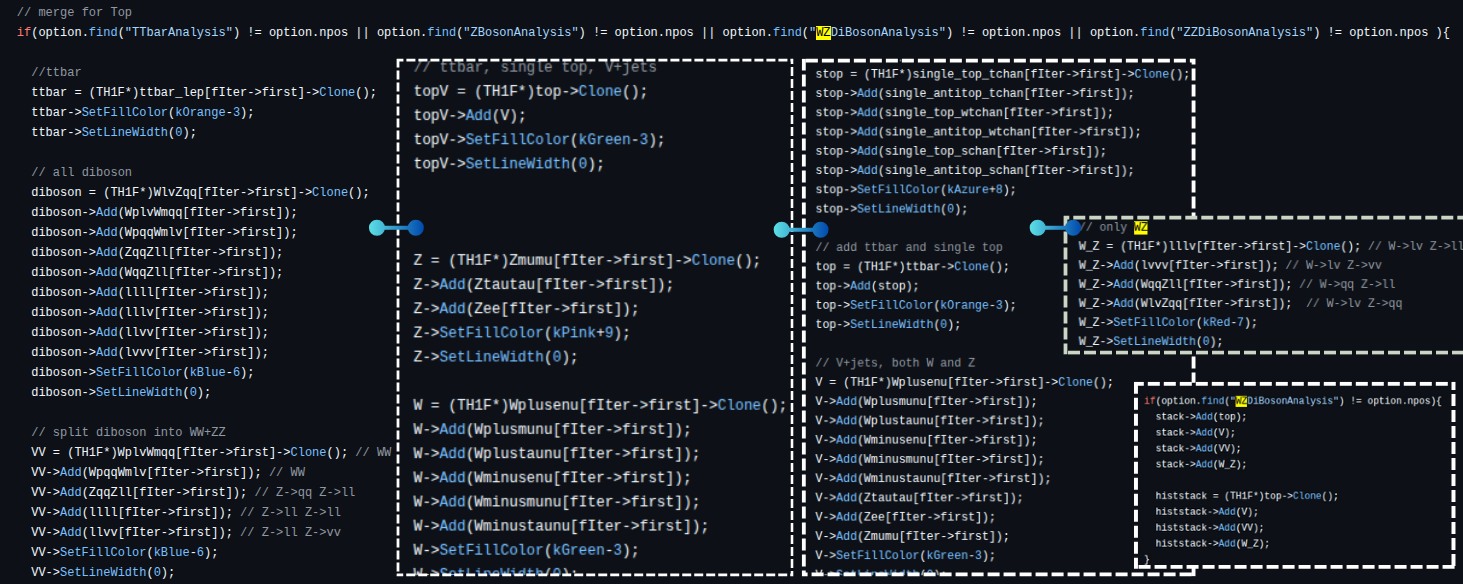
\includegraphics[width=\textwidth]{IMAGES/united.png}
    \caption{Example code screen shots of the \texttt{Plotting.cxx} script. Those lines should give you hints about the data and simulations you need to combine. This is for the WZ analysis, but similarly, you can find the same lines for other analysis.}
    \label{fig:united}
\end{figure}

\subsection*{1. Combining \texttt{.root} Files}
\begin{itemize}
    \item Use the \texttt{hadd} command to combine \texttt{.root} files generated by the ADL (Analysis Description Language) analysis. These files should be named appropriately (e.g., \texttt{data.root}, \texttt{V.root}, \texttt{VV.root}, etc.) to match the expected input for the \texttt{plot\_all.py} script.
    \item Example commands for combining files:
\end{itemize}

\begin{lstlisting}[language=bash]
hadd data.root file1.root file2.root file3.root
\end{lstlisting}

\begin{lstlisting}[language=bash]
hadd data.root file*.root
\end{lstlisting}

As a reference, you can find example commands in the \texttt{hadd.sh} script under the \url{https://github.com/ibeuler/CutLang-exercise-analysis} repository.

\subsection*{2. Setting Up the \texttt{plot\_all.py} Script}
\begin{itemize}
    \item The script is designed to handle different analyses (e.g., \texttt{WZ}, \texttt{Zboson}, \texttt{HZZ}, etc.) based on the \texttt{analysis\_name} parameter passed as a command-line argument.
    \item The script reads the combined \texttt{.root} files and extracts histograms for specific regions and variables.
\end{itemize}

\subsection*{3. Defining Variables to Plot}
\begin{itemize}
    \item At the bottom of the script, specific variables to be plotted are defined for each analysis. For example, for the \texttt{WZ} analysis, the following variables are defined:
\end{itemize}

\begin{lstlisting}[language=python]
#plotting("WZDiBoson","hist_etmiss",350)
#plotting("WZDiBoson","hist_threelepteta",600)
#plotting("WZDiBoson","hist_threeleptphi",400)
#plotting("WZDiBoson","hist_threeleptpt",1900)
#plotting("WZDiBoson","hist_threeleptE",1100)
#plotting("WZDiBoson","hist_mtw",400)
#plotting("WZDiBoson","hist_mLL",400)
plotting("WZDiBoson","hist_ptLL",400)
\end{lstlisting}

\begin{itemize}
    \item Uncomment the desired line(s) to plot specific variables.
\end{itemize}

\subsection*{4. Running the Script}
\begin{itemize}
    \item Execute the script with the appropriate analysis name using the \texttt{-a} or \texttt{--analysis} option. For example:
\end{itemize}

\begin{lstlisting}[language=bash]
python plot_all.py -a WZ
\end{lstlisting}

\subsection*{5. Plotting Histograms}
\begin{itemize}
    \item The script reads the histograms from the \texttt{.root} files, applies any necessary scaling, and stacks them for visualization.
    \item It uses ROOT's \texttt{THStack} to overlay histograms for different components (e.g., data, signal, background) and displays them in a single plot.
\end{itemize}

\subsection*{6. Customizing the Output}
\begin{itemize}
    \item The script includes options for setting axis labels, titles, and ranges. It also calculates ratios (e.g., Data/MC) and adds legends for clarity.
    \item The final plots are displayed and can be saved as images or PDFs.
\end{itemize}

\subsection*{7. Ensuring Proper Histogram and Region Naming in the ADL File}
\begin{itemize}
    \item The \texttt{plot\_all.py} script expects histograms and regions to follow specific naming conventions. Ensure that both histograms and regions are named correctly in the ADL file to match the script's requirements.
    \item For example, histograms for the \texttt{WZ} analysis should be named as follows:
\end{itemize}

\begin{lstlisting}[language=tex]
histogram hist_etmiss { ... }
histogram hist_threelepteta { ... }
histogram hist_threeleptphi { ... }
histogram hist_threeleptpt { ... }
histogram hist_threeleptE { ... }
histogram hist_mtw { ... }
histogram hist_mLL { ... }
histogram hist_ptLL { ... }
\end{lstlisting}

\begin{itemize}
    \item Similarly, regions should also follow specific naming conventions.
\end{itemize}

\begin{itemize}
    \item Verify that the histogram and region names in the ADL file match the names used in the \texttt{plotting()} function calls and other parts of the \texttt{plot\_all.py} script.
    \item Consistent naming ensures that the script can correctly locate and process the histograms and regions for plotting.
\end{itemize}

By following this process, you can visualize the results of your analysis for the desired variables and compare different components in a single plot.

\end{document}